\documentclass[compress,aspectratio=169]{beamer}
\usepackage{irbookslide}
\usepackage{irilmenau2}
\usepackage{tikz}
\usepackage{url}
\usepackage{ifxetex}
%\RequireXeTeX
\usepackage{fontspec} % zahteva paket euenc
\usepackage{xunicode}
\usepackage{xltxtra}
\usepackage{polyglossia}
\usepackage{minted}
\usepackage[noend]{algorithmic}
\renewcommand{\algorithmicrequire}{\textbf{Input:}}
\renewcommand{\algorithmicensure}{\textbf{Output:}}
\renewcommand{\algorithmiccomment}[1]{\hfill \{\myred{#1}\}}
\usepackage{xcolor,colortbl}
\usepackage{textcomp}
\usepackage{unicode-math}
%\usepackage{hyphenat}
%\setdefaultlanguage[script=Latin]{serbian}

\title{Projekat 1}
\author{Branko Milosavljević}
\institute{Katedra za informatiku, Fakultet tehničkih nauka, Univerzitet u
Novom Sadu}
\date{2022.}
\subject{Predavanja sa ASP}

\begin{document}

\frame{\titlepage}

\section[Aritmetički izrazi]{Izračunavanje aritmetičkih izraza}

\begin{frame}[fragile]
  \frametitle{Infiksna, postfiksna, prefiksna notacija}
  \begin{itemize}
    \item infiksna notacija: $x + y$
    \item postfiksna notacija: $x y +$
    \item prefiksna notacija: $+ x y$
  \end{itemize}
\end{frame}

\begin{frame}[fragile]
  \frametitle{Infiksna, postfiksna, prefiksna notacija}
  \begin{center}
    \begin{tabular}{l|l|l}
      \textbf{infix} & \textbf{postfix} & \textbf{prefix} \\ \hline
      $a * b + c / d$ & $a b * c d / +$ & $+ * a b / c d$ \\ \hline
      $a * (b + c) / d$ & $a b c + * d /$ & $/ * a + b c d$ \\ \hline
      $a * (b + c / d)$ & $ a b c d / + *$ & $* a + b / c d$
    \end{tabular}
  \end{center}
\end{frame}
  
\begin{frame}[fragile]
  \frametitle{Stablo izraza}
  \begin{itemize}
    \item $a * b + c / d$
  \end{itemize}
  \begin{center}
    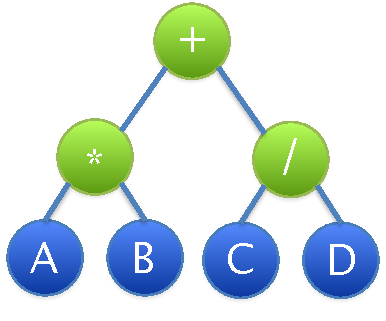
\includegraphics[width=5cm]{prj-01-pic01.pdf}
  \end{center}
\end{frame}
    
\begin{frame}[fragile]
  \frametitle{Konverzija infix $\rightarrow$ postfix}
  \begin{itemize}
    \item interno koristimo stek
    \item izraz u obliku stringa se parsira u listu tokena
    \item rezultat je izlazna lista
    \item prolazimo kroz listu tokena sleva u desno
    \begin{enumerate}
      \item token je operand: dodaj u izlaznu listu
      \item token je leva zagrada: dodaj na stek
      \item token je desna zagrada: skidaj sa steka i dodaj u listu do prve leve zagrade; zagradu ukloni
      \item token je operator: skini operatore sa steka koji imaju veći ili jednak prioritet; dodaj operator na stek
    \end{enumerate}
    \item isprazni stek dodavanjem u listu
  \end{itemize}
\end{frame}

\begin{frame}[fragile]
  \frametitle{Primer 1: infix $\rightarrow$ postfix}
  \begin{itemize}
    \only<1>{
      \item izraz: 3 + 4 * 5 / 6
      \item stek:
      \item izlaz:
    }
    \only<2>{
      \item izraz: \textbf{\myred{3}} + 4 * 5 / 6
      \item stek:
      \item izlaz:  
    }
    \only<3>{
      \item izraz: 3 \textbf{\myred{+}} 4 * 5 / 6
      \item stek: 
      \item izlaz: 3
    }
    \only<4>{
      \item izraz: 3 + \textbf{\myred{4}} * 5 / 6
      \item stek: +
      \item izlaz: 3
    }
    \only<5>{
      \item izraz: 3 + 4 \textbf{\myred{*}} 5 / 6
      \item stek: +
      \item izlaz: 3 4
    }
    \only<6>{
      \item izraz: 3 + 4 * \textbf{\myred{5}} / 6
      \item stek: + *
      \item izlaz: 3 4
    }
    \only<7>{
      \item izraz: 3 + 4 * 5 \textbf{\myred{/}} 6
      \item stek: + *
      \item izlaz: 3 4 5
    }
    \only<8>{
      \item izraz: 3 + 4 * 5 \textbf{\myred{/}} 6
      \item stek: + 
      \item izlaz: 3 4 5 *        
    }
    \only<9>{
      \item izraz: 3 + 4 * 5 / \textbf{\myred{6}}
      \item stek: + /
      \item izlaz: 3 4 5 *  
    }
    \only<10>{
      \item izraz: 3 + 4 * 5 / 6
      \item stek: + /
      \item izlaz: 3 4 5 * 6  
    }
    \only<11>{
      \item izraz: 3 + 4 * 5 / 6
      \item stek: +
      \item izlaz: 3 4 5 * 6 /  
    }
    \only<12>{
      \item izraz: 3 + 4 * 5 / 6
      \item stek:
      \item izlaz: 3 4 5 * 6 / +
      \item kraj!  
    }
  \end{itemize}
\end{frame}

\begin{frame}[fragile]
  \frametitle{Primer 2: infix $\rightarrow$ postfix}
  \begin{itemize}
    \only<1>{
      \item izraz: (4 + 8) * (6 - 5) / ((3 - 2) * (2 + 2))
      \item stek:
      \item izlaz:
    }
    \only<2>{
      \item izraz: \textbf{\myred{(}}4 + 8) * (6 - 5) / ((3 - 2) * (2 + 2))
      \item stek:
      \item izlaz:  
    }
    \only<3>{
      \item izraz: (\textbf{\myred{4}} + 8) * (6 - 5) / ((3 - 2) * (2 + 2))
      \item stek: (
      \item izlaz: 
    }
    \only<4>{
      \item izraz: (4 \textbf{\myred{+}} 8) * (6 - 5) / ((3 - 2) * (2 + 2))
      \item stek: (
      \item izlaz: 4
    }
    \only<5>{
      \item izraz: (4 + \textbf{\myred{8}}) * (6 - 5) / ((3 - 2) * (2 + 2))
      \item stek: ( +
      \item izlaz: 4
    }
    \only<6>{
      \item izraz: (4 + 8\textbf{\myred{)}} * (6 - 5) / ((3 - 2) * (2 + 2))
      \item stek: ( +
      \item izlaz: 4 8
    }
    \only<7>{
      \item izraz: (4 + 8\textbf{\myred{)}} * (6 - 5) / ((3 - 2) * (2 + 2))
      \item stek: (
      \item izlaz: 4 8 +
    }
    \only<8>{
      \item izraz: (4 + 8) \textbf{\myred{*}} (6 - 5) / ((3 - 2) * (2 + 2))
      \item stek: 
      \item izlaz: 4 8 +
    }
    \only<9>{
      \item izraz: (4 + 8) * \textbf{\myred{(}} 6 - 5) / ((3 - 2) * (2 + 2))
      \item stek: *
      \item izlaz: 4 8 +
    }
    \only<10>{
      \item izraz: (4 + 8) * (\textbf{\myred{6}} - 5) / ((3 - 2) * (2 + 2))
      \item stek: * (
      \item izlaz: 4 8 +
    }
    \only<11>{
      \item izraz: (4 + 8) * (6 \textbf{\myred{-}} 5) / ((3 - 2) * (2 + 2))
      \item stek: * (
      \item izlaz: 4 8 + 6
    }
    \only<12>{
      \item izraz: (4 + 8) * (6 - \textbf{\myred{5}}) / ((3 - 2) * (2 + 2))
      \item stek: * ( -
      \item izlaz: 4 8 + 6
    }
    \only<13>{
      \item izraz: (4 + 8) * (6 - 5\textbf{\myred{)}} / ((3 - 2) * (2 + 2))
      \item stek: * ( -
      \item izlaz: 4 8 + 6 5
    }
    \only<14>{
      \item izraz: (4 + 8) * (6 - 5\textbf{\myred{)}} / ((3 - 2) * (2 + 2))
      \item stek: * (
      \item izlaz: 4 8 + 6 5 -
    }
    \only<15>{
      \item izraz: (4 + 8) * (6 - 5) \textbf{\myred{/}} ((3 - 2) * (2 + 2))
      \item stek: *
      \item izlaz: 4 8 + 6 5 -
    }
    \only<16>{
      \item izraz: (4 + 8) * (6 - 5) \textbf{\myred{/}} ((3 - 2) * (2 + 2))
      \item stek: 
      \item izlaz: 4 8 + 6 5 - *
    }
    \only<17>{
      \item izraz: (4 + 8) * (6 - 5) / \textbf{\myred{(}} (3 - 2) * (2 + 2))
      \item stek: /
      \item izlaz: 4 8 + 6 5 - *
    }
    \only<18>{
      \item izraz: (4 + 8) * (6 - 5) / ( \textbf{\myred{(}} 3 - 2) * (2 + 2))
      \item stek: / (
      \item izlaz: 4 8 + 6 5 - *
    }
    \only<19>{
      \item izraz: (4 + 8) * (6 - 5) / (( \textbf{\myred{3}} - 2) * (2 + 2))
      \item stek: / ( (
      \item izlaz: 4 8 + 6 5 - *
    }
    \only<20>{
      \item izraz: (4 + 8) * (6 - 5) / ((3 \textbf{\myred{-}} 2) * (2 + 2))
      \item stek: / ( (
      \item izlaz: 4 8 + 6 5 - * 3
    }
    \only<21>{
      \item izraz: (4 + 8) * (6 - 5) / ((3 - \textbf{\myred{2}}) * (2 + 2))
      \item stek: / ( ( -
      \item izlaz: 4 8 + 6 5 - * 3
    }
    \only<22>{
      \item izraz: (4 + 8) * (6 - 5) / ((3 - 2\textbf{\myred{)}} * (2 + 2))
      \item stek: / ( ( -
      \item izlaz: 4 8 + 6 5 - * 3 2
    }
    \only<23>{
      \item izraz: (4 + 8) * (6 - 5) / ((3 - 2\textbf{\myred{)}} * (2 + 2))
      \item stek: / ( (
      \item izlaz: 4 8 + 6 5 - * 3 2 -
    }
    \only<24>{
      \item izraz: (4 + 8) * (6 - 5) / ((3 - 2) \textbf{\myred{*}} (2 + 2))
      \item stek: / (
      \item izlaz: 4 8 + 6 5 - * 3 2 -
    }
    \only<25>{
      \item izraz: (4 + 8) * (6 - 5) / ((3 - 2) * \textbf{\myred{(}} 2 + 2))
      \item stek: / ( *
      \item izlaz: 4 8 + 6 5 - * 3 2 -
    }
    \only<26>{
      \item izraz: (4 + 8) * (6 - 5) / ((3 - 2) * (\textbf{\myred{2}} + 2))
      \item stek: / ( * (
      \item izlaz: 4 8 + 6 5 - * 3 2 -
    }
    \only<27>{
      \item izraz: (4 + 8) * (6 - 5) / ((3 - 2) * (2 \textbf{\myred{+}} 2))
      \item stek: / ( * (
      \item izlaz: 4 8 + 6 5 - * 3 2 - 2
    }
    \only<28>{
      \item izraz: (4 + 8) * (6 - 5) / ((3 - 2) * (2 + \textbf{\myred{2}}))
      \item stek: / ( * ( +
      \item izlaz: 4 8 + 6 5 - * 3 2 - 2
    }
    \only<29>{
      \item izraz: (4 + 8) * (6 - 5) / ((3 - 2) * (2 + 2 \textbf{\myred{)}})
      \item stek: / ( * ( +
      \item izlaz: 4 8 + 6 5 - * 3 2 - 2 2
    }
    \only<30>{
      \item izraz: (4 + 8) * (6 - 5) / ((3 - 2) * (2 + 2 \textbf{\myred{)}})
      \item stek: / ( * (
      \item izlaz: 4 8 + 6 5 - * 3 2 - 2 2 +
    }
    \only<31>{
      \item izraz: (4 + 8) * (6 - 5) / ((3 - 2) * (2 + 2)\textbf{\myred{)}}
      \item stek: / ( *
      \item izlaz: 4 8 + 6 5 - * 3 2 - 2 2 +
    }
    \only<32>{
      \item izraz: (4 + 8) * (6 - 5) / ((3 - 2) * (2 + 2)\textbf{\myred{)}}
      \item stek: / (
      \item izlaz: 4 8 + 6 5 - * 3 2 - 2 2 + *
    }
    \only<33>{
      \item izraz: (4 + 8) * (6 - 5) / ((3 - 2) * (2 + 2))
      \item stek: /
      \item izlaz: 4 8 + 6 5 - * 3 2 - 2 2 + *
    }
    \only<34>{
      \item izraz: (4 + 8) * (6 - 5) / ((3 - 2) * (2 + 2))
      \item stek: 
      \item izlaz: 4 8 + 6 5 - * 3 2 - 2 2 + * /
      \item kraj!
    }
  \end{itemize}
\end{frame}

\section{Slagalica}

\begin{frame}[fragile]
  \frametitle{Rešavanje slagalice}
  \begin{itemize}
    \item promešana slagalica
  \end{itemize}
  \begin{center}
    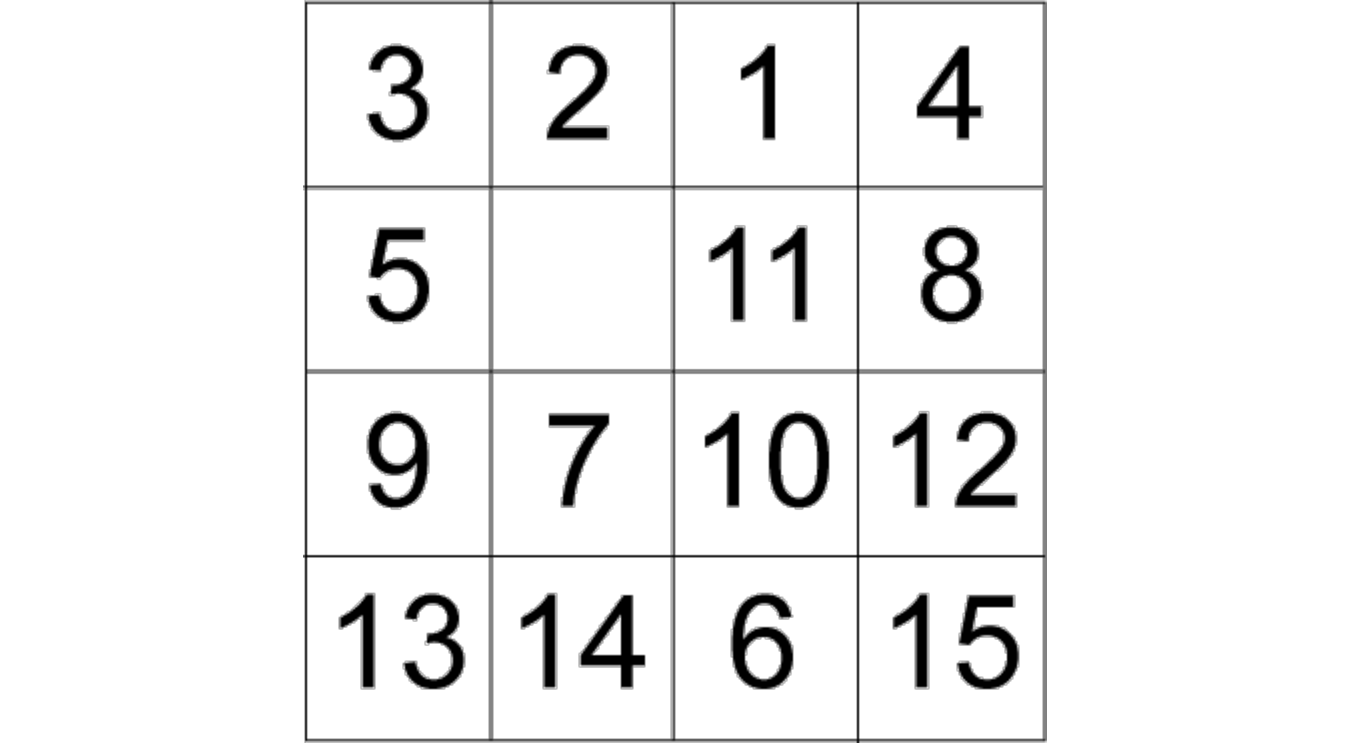
\includegraphics[width=10cm]{prj-01-pic02.pdf}
  \end{center}
\end{frame}

\begin{frame}[fragile]
  \frametitle{Rešavanje slagalice}
  \begin{itemize}
    \item rešena slagalica
  \end{itemize}
  \begin{center}
    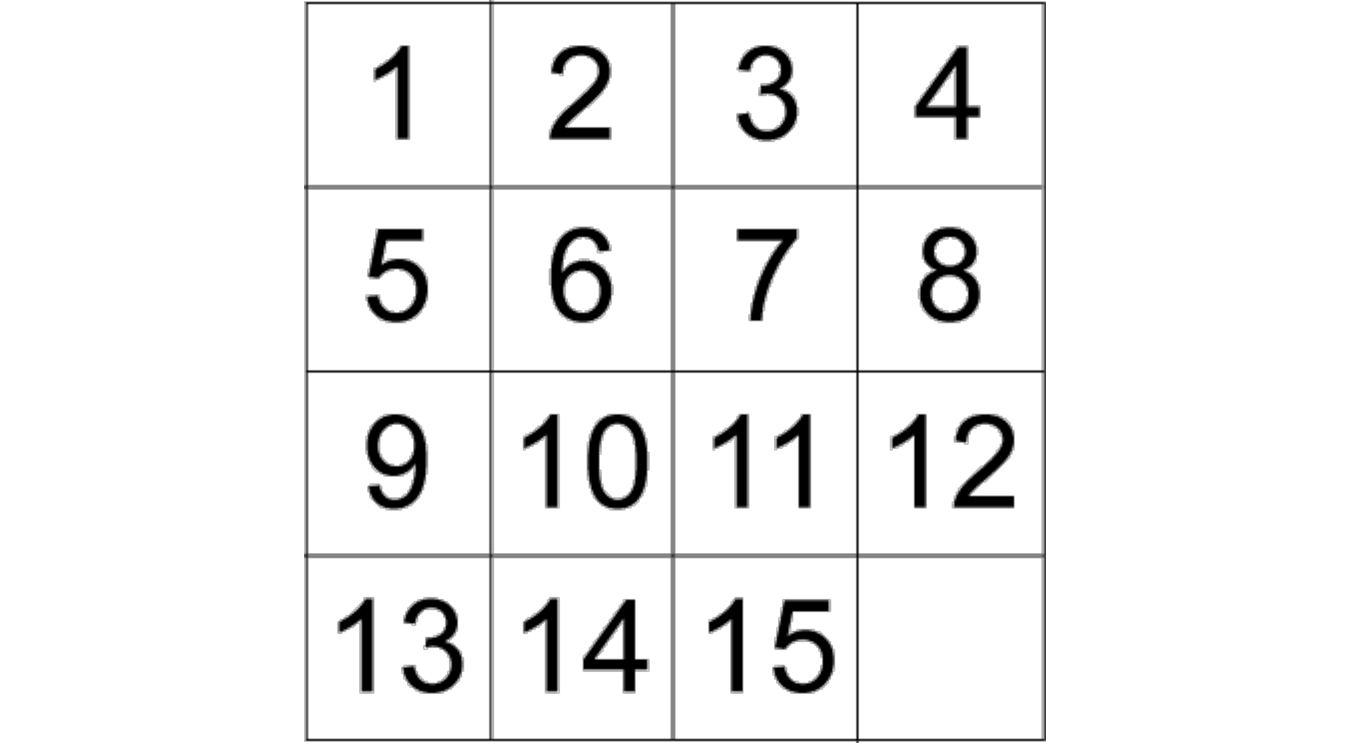
\includegraphics[width=10cm]{prj-01-pic03.pdf}
  \end{center}
\end{frame}

\begin{frame}[fragile]
  \frametitle{Jedan potez u rešavanju}
  \begin{center}
    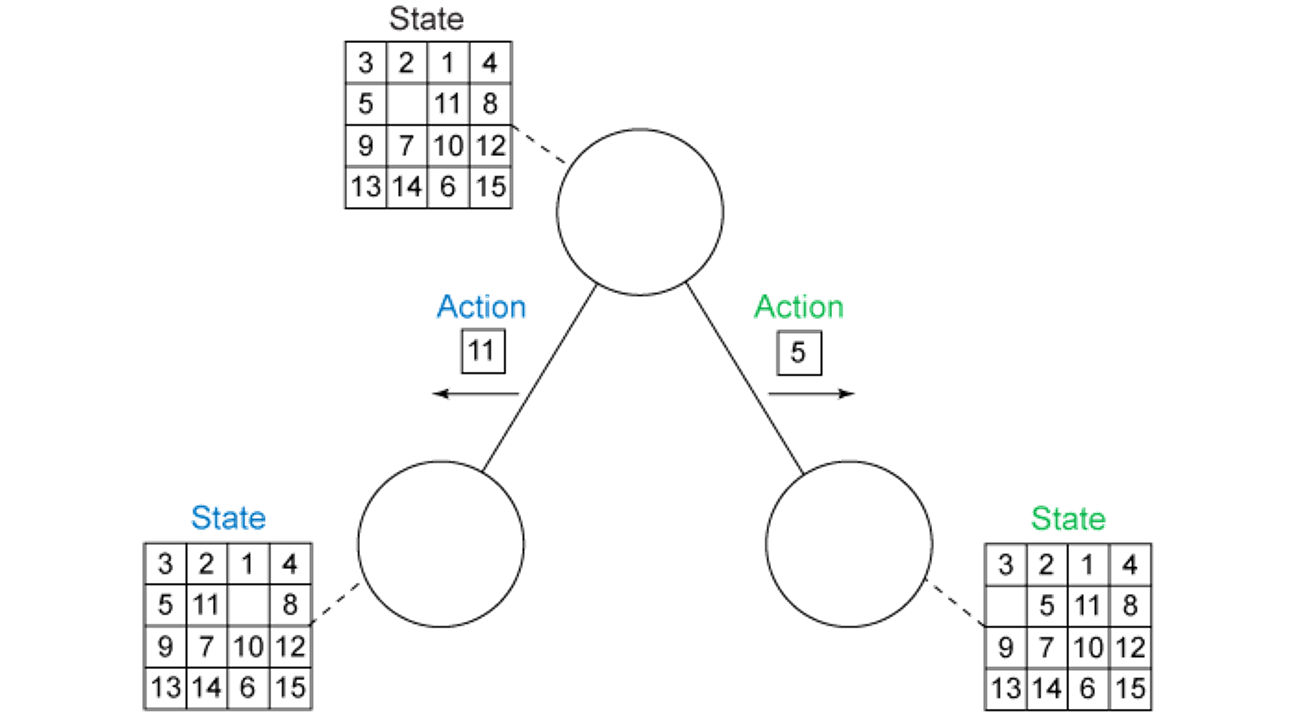
\includegraphics[width=8cm]{prj-01-pic04.png}
  \end{center}
\end{frame}

\begin{frame}[fragile]
  \frametitle{Procena udaljenosti od cilja}
  \begin{itemize}
    \item $g$: broj pređenih poteza
    \item $h$: procena broja preostalih poteza
  \end{itemize}
  \begin{center}
    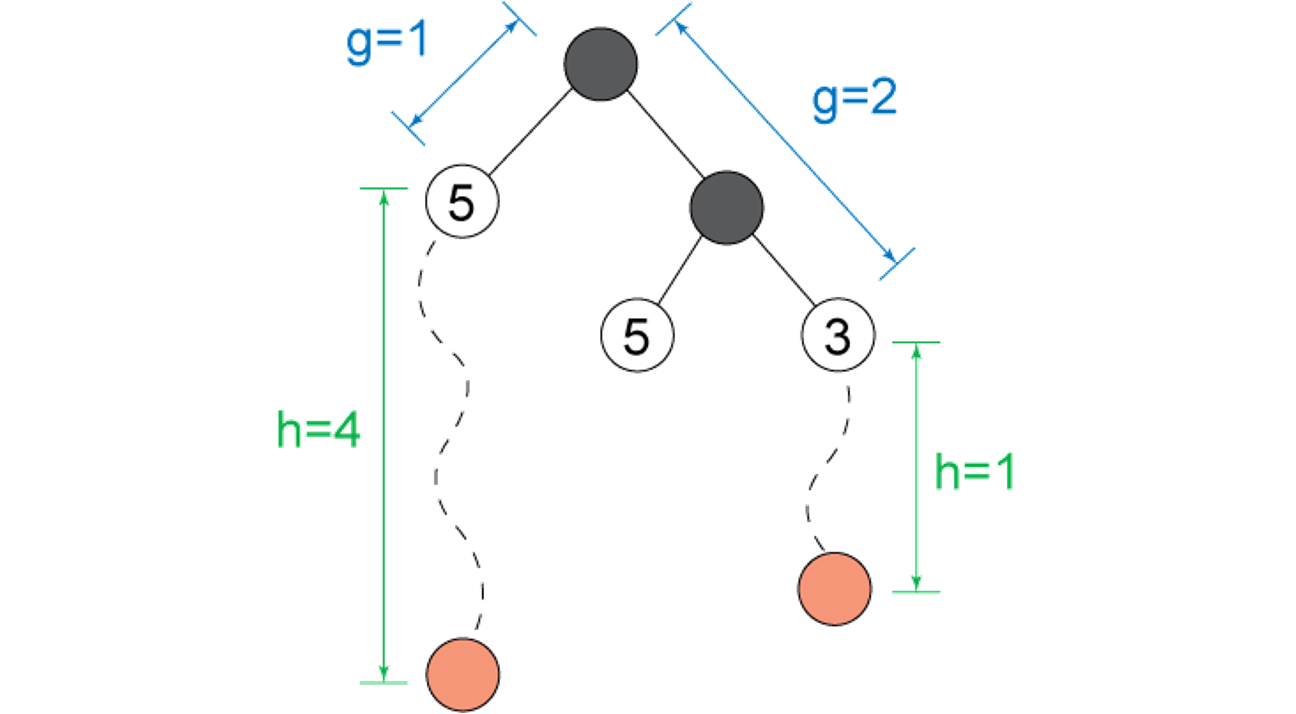
\includegraphics[width=10cm]{prj-01-pic05.png}
  \end{center}
\end{frame}

\begin{frame}[fragile]
  \frametitle{Procena broja preostalih poteza}
  \begin{itemize}
    \item Hamming rastojanje
    \begin{itemize}
      \item broj pločica koje nisu na svom mestu
    \end{itemize}
    \item Manhattan rastojanje
    \begin{itemize}
      \item udaljenost pločice od svog konačnog mesta, po horizontali + po vertikali
      \item suma za sve pločice
    \end{itemize}
  \end{itemize}
\end{frame}

\begin{frame}[fragile]
  \frametitle{Best-first kretanje po stablu}
  \begin{center}
    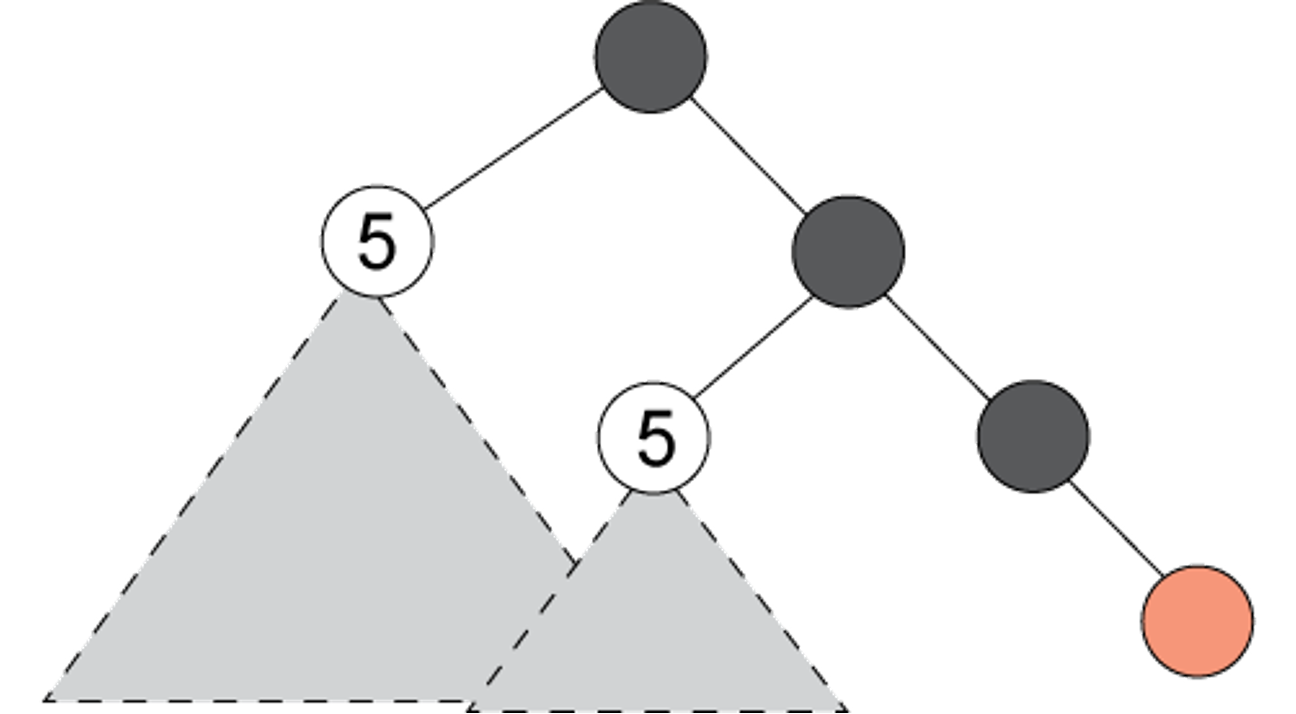
\includegraphics[width=10cm]{prj-01-pic06.png}
  \end{center}
\end{frame}

\begin{frame}[fragile]
  \frametitle{A*-search}
  \begin{verbatim}
    function: A*-search(initial)
    open <- priority_queue{initial}
    closed <- queue{}
    while not_empty(open):
        node <- best(open)
        if node.is_final():
            return solution(node)
        if node in closed:
            continue
        closed.add(node)
        for next_node in actions(node):
            open.add(next_node)    
  \end{verbatim}
\end{frame}

\section{Mice}

\begin{frame}[fragile]
  \frametitle{Mice (Nine men's morris) i $\alpha-\beta$ rezanje}
  \begin{itemize}
    \item treba naći putanju od početne do krajnje pozicije
    \item kod slagalice mi igramo \textbf{svaki} potez
    \item igre sa 2 igrača se igraju naizmenično
    \item drugi igrač ima suprotan cilj od nas
    \item pretraga se mora drugačije raditi
  \end{itemize}
\end{frame}

\begin{frame}[fragile]
  \frametitle{Mice (Nine men's morris) i $\alpha-\beta$ rezanje}
  \begin{itemize}
    \item svaki završetak igre ima \textbf{rezultat} koji ćemo predstaviti brojem
    \item volimo pozitivne brojeve
    \item kod nekih igara: \\ +1 je pobeda, 0 je nerešeno, -1 je poraz
    \item kod nekih drugih ne mora biti 1/0/-1 \\ npr. količina novca osvojenog u pokeru
  \end{itemize}
\end{frame}

\begin{frame}[fragile]
  \frametitle{Igre sa nultom sumom}
  \begin{itemize}
    \item ono što mi osvojimo plus ono što osvoji protivnik je uvek jednako 0
    \item za nas -- pozitivni brojevi su dobri a negativni loši
    \item za protivnika -- obrnuto
  \end{itemize}
\end{frame}

\begin{frame}[fragile]
  \frametitle{Primer trivijalne igre}
  \begin{columns}
    \column{8cm}
    \begin{itemize}
      \item želimo da osvojimo 50
      \item da li je to realno?
      \item kako da odigramo?
    \end{itemize}
    \column{8cm}
    \begin{center}
      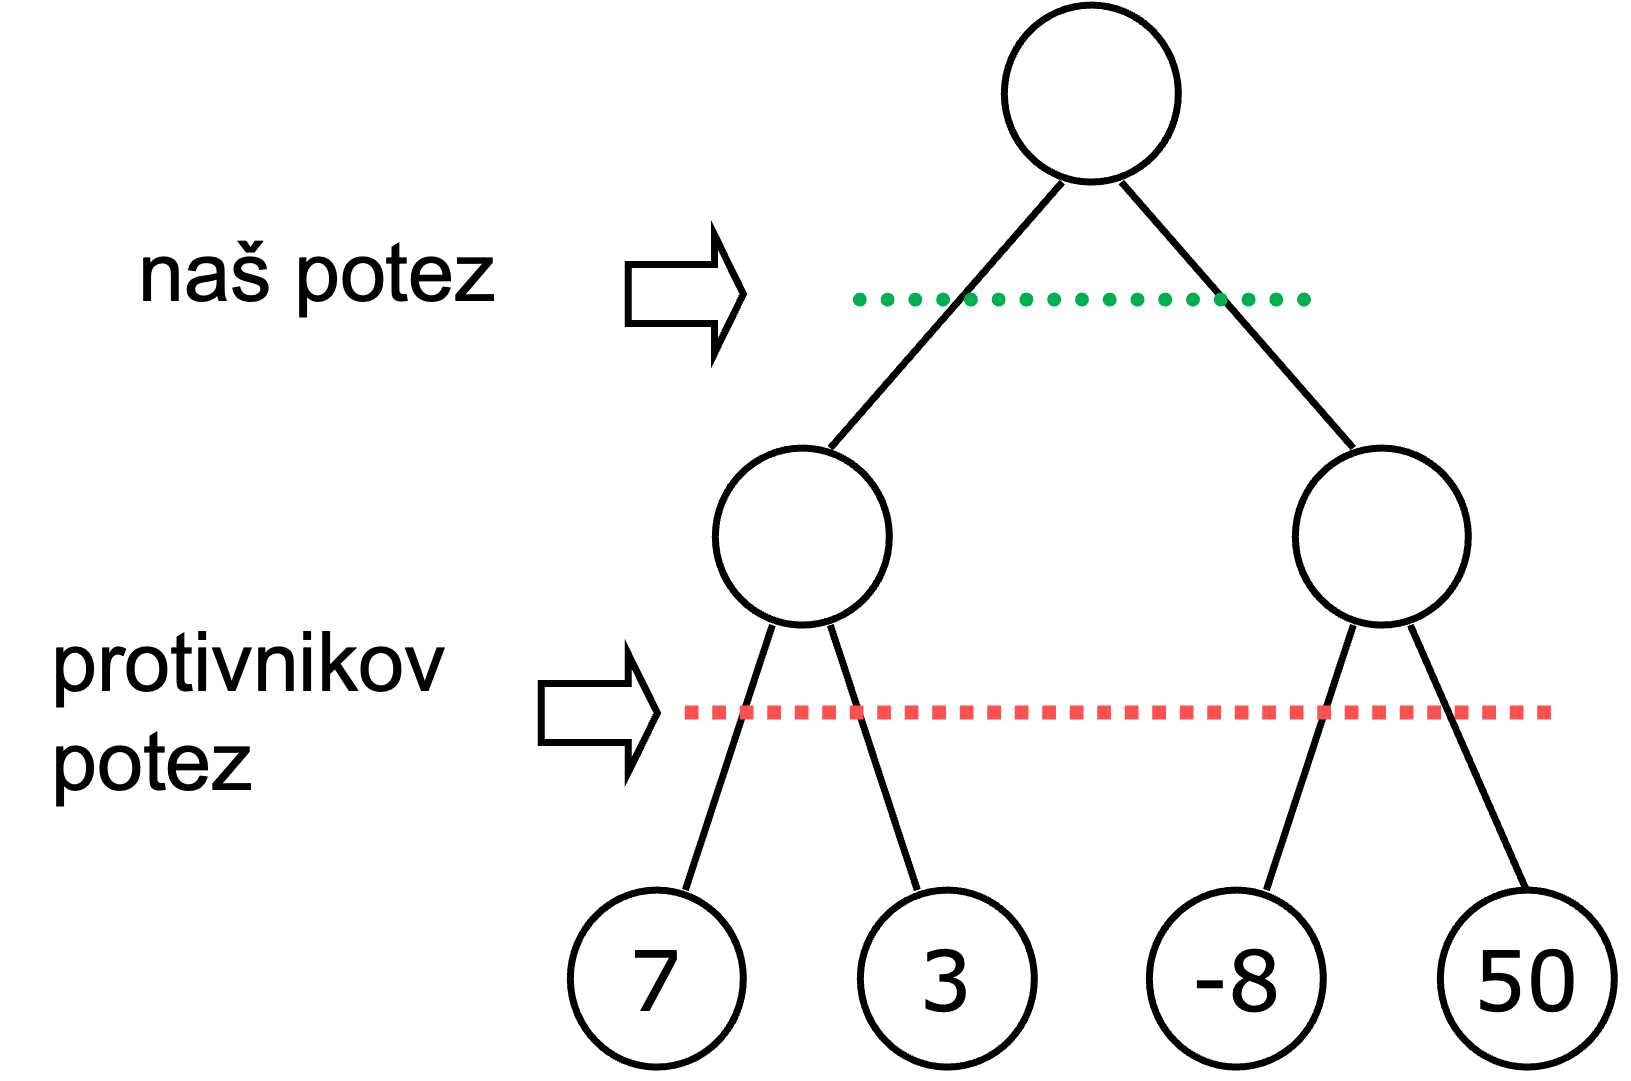
\includegraphics[width=7cm]{prj-01-pic07.png}
    \end{center}
\end{columns}
\end{frame}

\begin{frame}[fragile]
  \frametitle{Minimax}
  \begin{columns}
    \column{8cm}
    \begin{itemize}
      \item protivnik će birati manje brojeve
      \item ako odigramo levo, protivnik će izabrati \textbf{\myred{3}}
      \item ako odigramo desno, protivnik će izabrati \textbf{\myred{-8}}
      \item dakle, biramo između \textbf{\myred{3}} i \textbf{\myred{-8}}
      \item igraćemo levo
    \end{itemize}
    \column{8cm}
    \begin{center}
      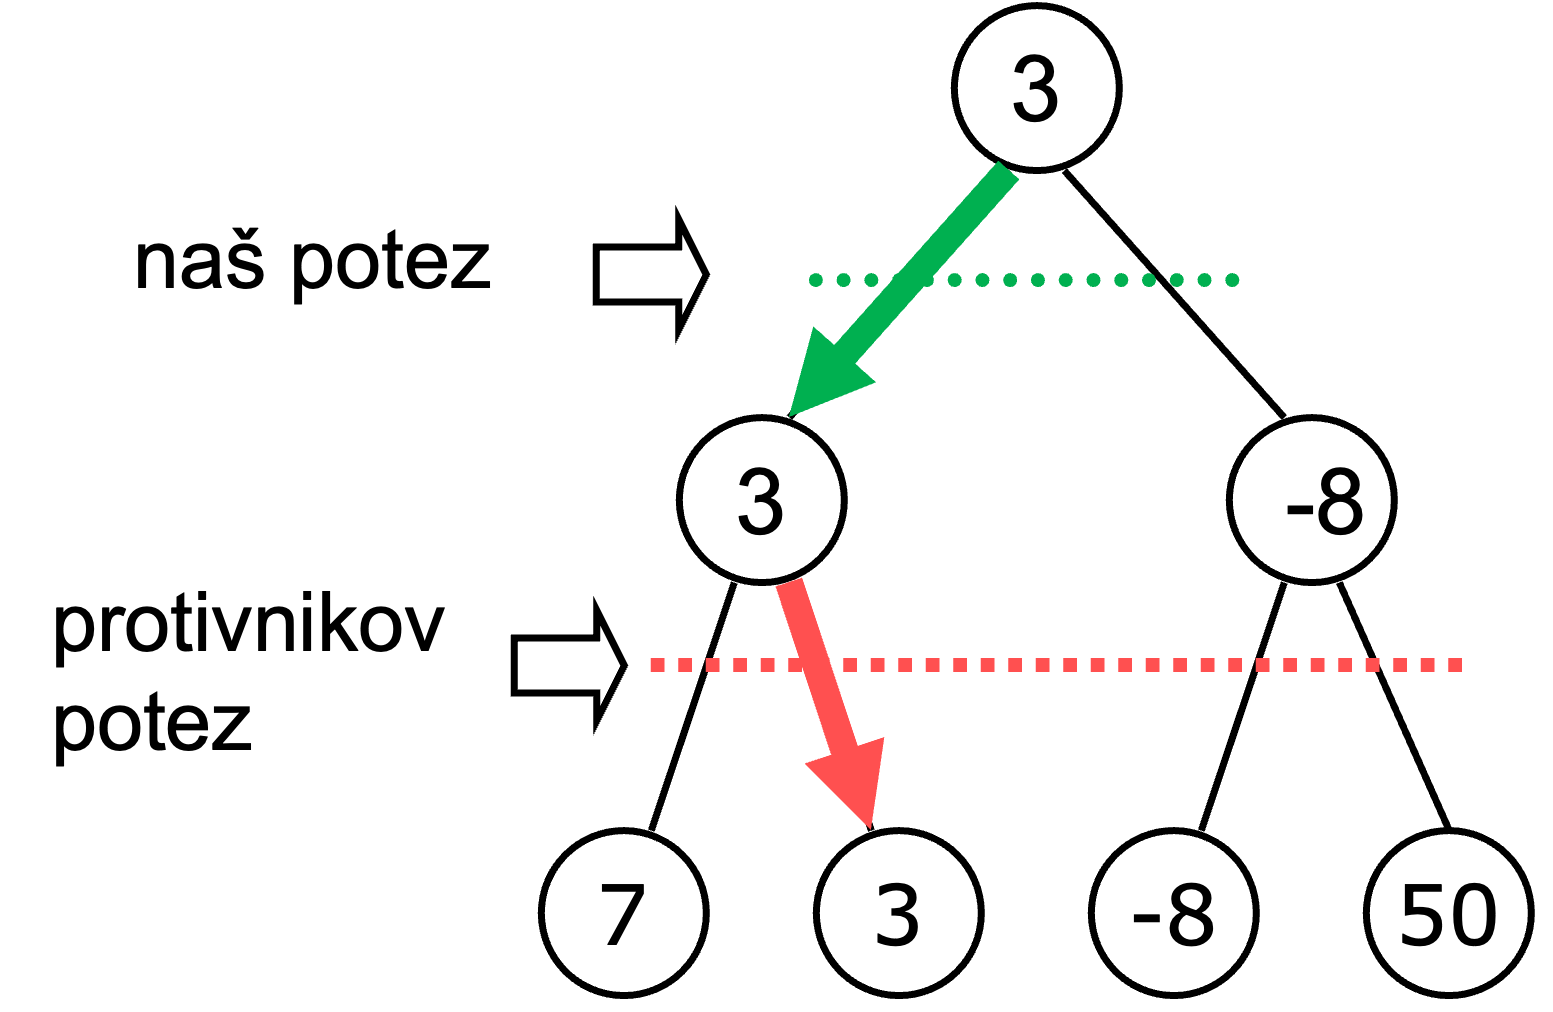
\includegraphics[width=7cm]{prj-01-pic08.png}
    \end{center}
  \end{columns}
\end{frame}

\begin{frame}[fragile]
  \frametitle{,,iks-oks`` / ,,puta-nula``}
  \begin{itemize}
    \item stablo igre nije veliko i možemo ga kompletnog izračunati
  \end{itemize}
  \begin{center}
    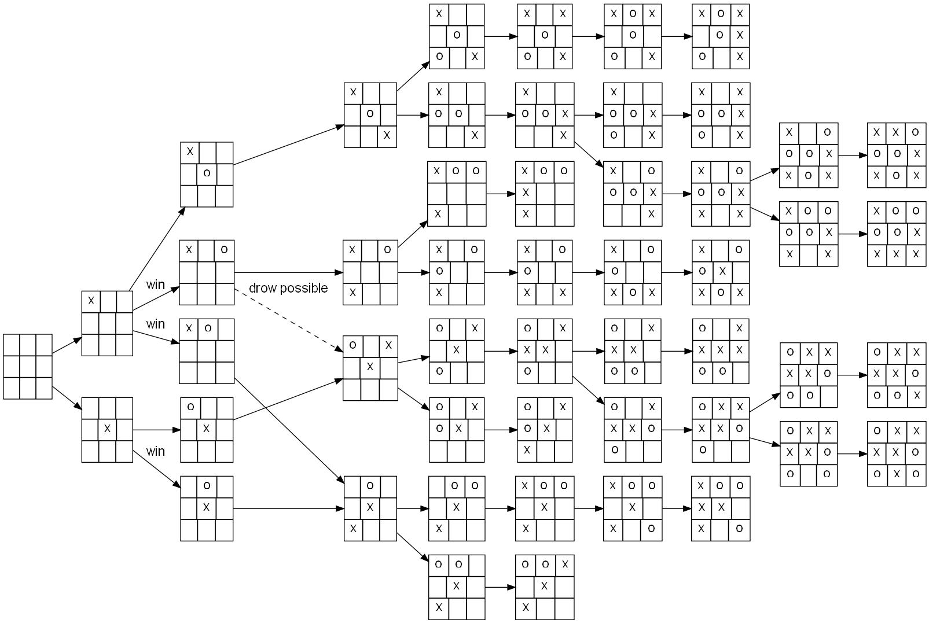
\includegraphics[width=9cm]{prj-01-pic09.png}
  \end{center}
\end{frame}

\begin{frame}[fragile]
  \frametitle{Heuristika}
  \begin{itemize}
    \item kada je stablo veliko ne znamo unapred ishode
    \item \textbf{heuristička funkcija} izračunava procenu dobitka za dati čvor u stablu
    \item pretpostavke
    \begin{itemize}
      \item protivnik će igrati u svoju korist
      \item što više poteza unapred analiziramo -- preciznija je procena
    \end{itemize}
  \end{itemize}
\end{frame}

\begin{frame}[fragile]
  \frametitle{Preliminarna vrednost čvora}
  \begin{itemize}
    \item idi niz stablo po dubini do zadatog broja nivoa
    \item za čvor na najnižem nivou izračunaj heuristiku
    \item za čvorove iz prethodnih nivoa:
    \begin{itemize}
      \item ako je \textbf{naš potez}, uzmi \textbf{najveću} vrednost od dece, eventualno pregazi prethodnu vrednost ako je manja
      \item ako je \textbf{protivnikov potez}, uzmi \textbf{najmanju} vrednost od dece, eventualno pregazi prethodnu vrednost ako je veća
    \end{itemize}
  \end{itemize}
\end{frame}

\begin{frame}[fragile]
  \frametitle{Primer}
  \begin{columns}
    \column{8cm}
    \begin{itemize}
      \item obilazak po dubini: dođi do lista, izračunaj 8, popni u roditelja
      \item idi na 5; manji je od 8, ignoriši
      \item vrati se gore, popni 8
      \item siđi u 2, popni je gore
      \item siđi u 9, popni je gore (9>2)
      \item 9 nije bolje od 8 za protivnika, ostavi 8
      \item siđi u -3, itd
    \end{itemize}
    \column{8cm}
    \begin{center}
      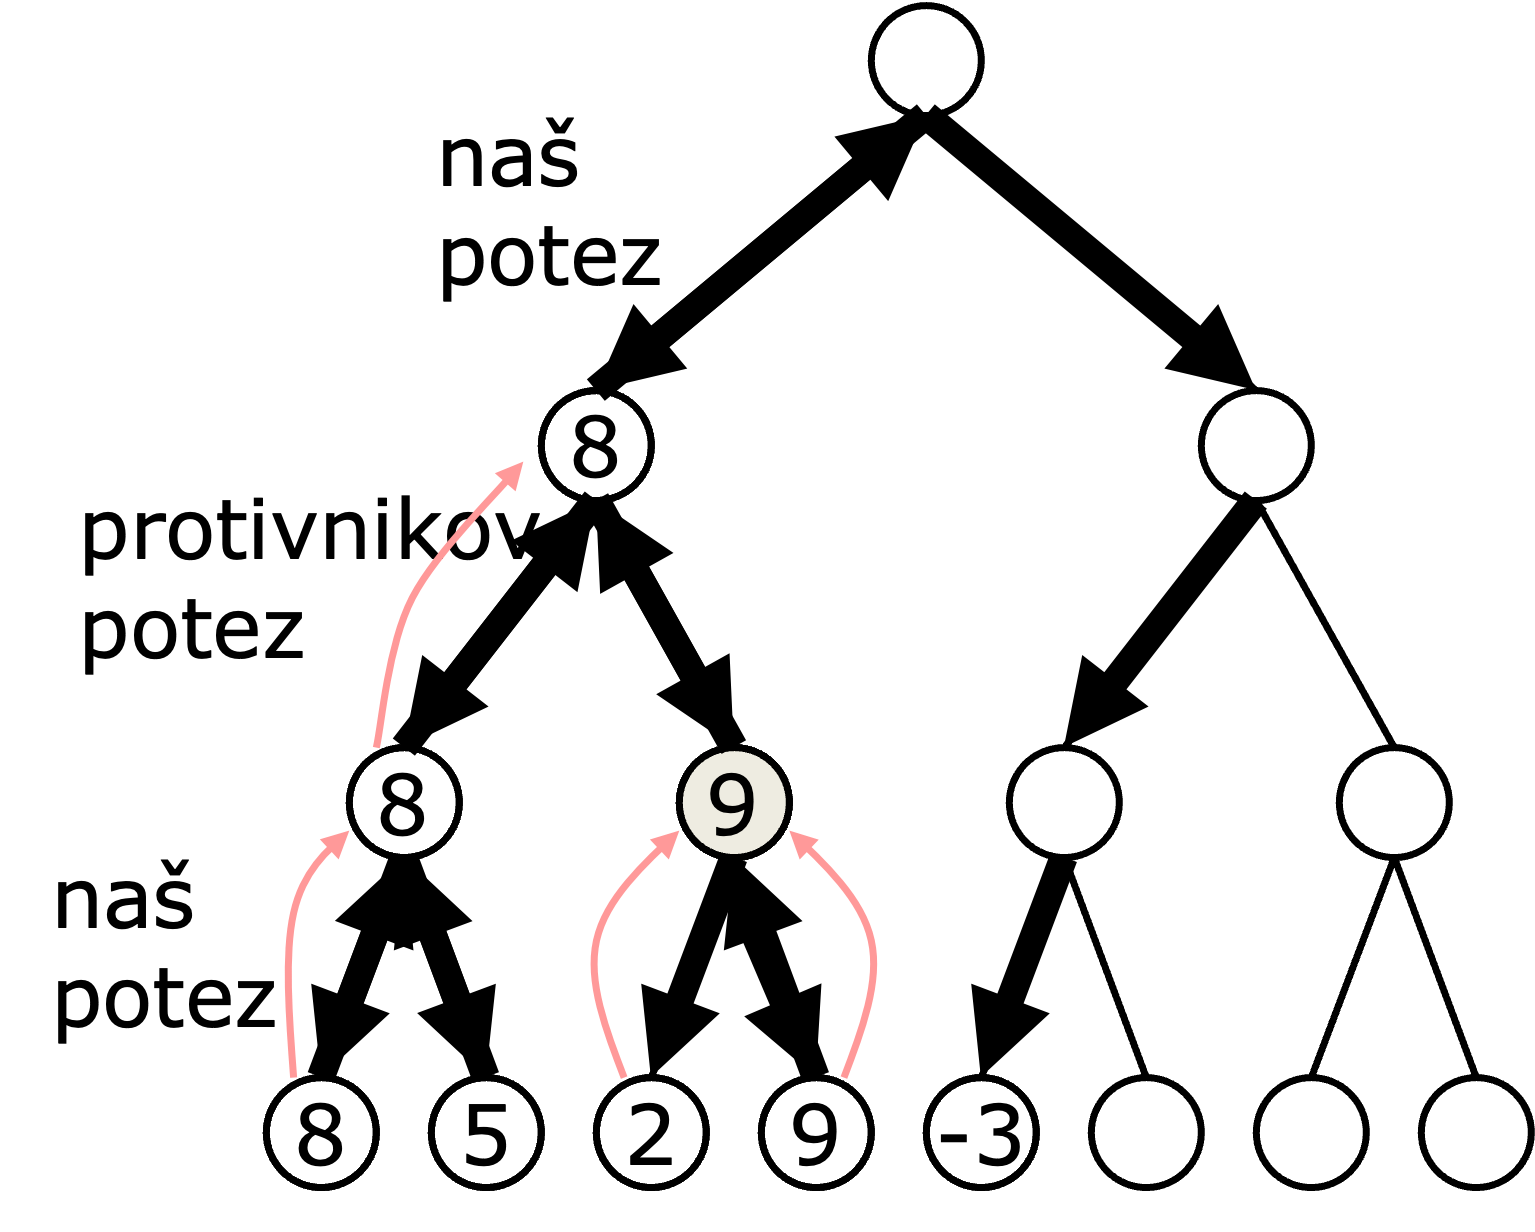
\includegraphics[width=7cm]{prj-01-pic10.png}
    \end{center}
  \end{columns}
\end{frame}

\begin{frame}[fragile]
  \frametitle{Penjanje vrednosti uz stablo}
  \begin{itemize}
    \item ako je naš potez:
    \begin{itemize}
      \item ako dete ima veću vrednost, iskopiraj je
    \end{itemize}
    \item ako je protivnikov potez:
    \begin{itemize}
      \item ako dete ima manju vrednost, iskopiraj je
    \end{itemize}
    \item na naš potez -- nikad ne smanjuj vrednost
    \item na protivnikov potez -- nikad ne povećavaj vrednost
  \end{itemize}
\end{frame}

\begin{frame}[fragile]
  \frametitle{Alfa rez}
  \begin{columns}
    \column{8cm}
    \begin{itemize}
      \item vrednost u korenu je za sada 8
      \item ako idemo desno vrednost je 1
      \item protivnik je nikad neće povećati na više od 1: uvek će biti manja od 8
      \item možemo ignorisati preostale čvorove
    \end{itemize}
    \column{8cm}
    \begin{center}
      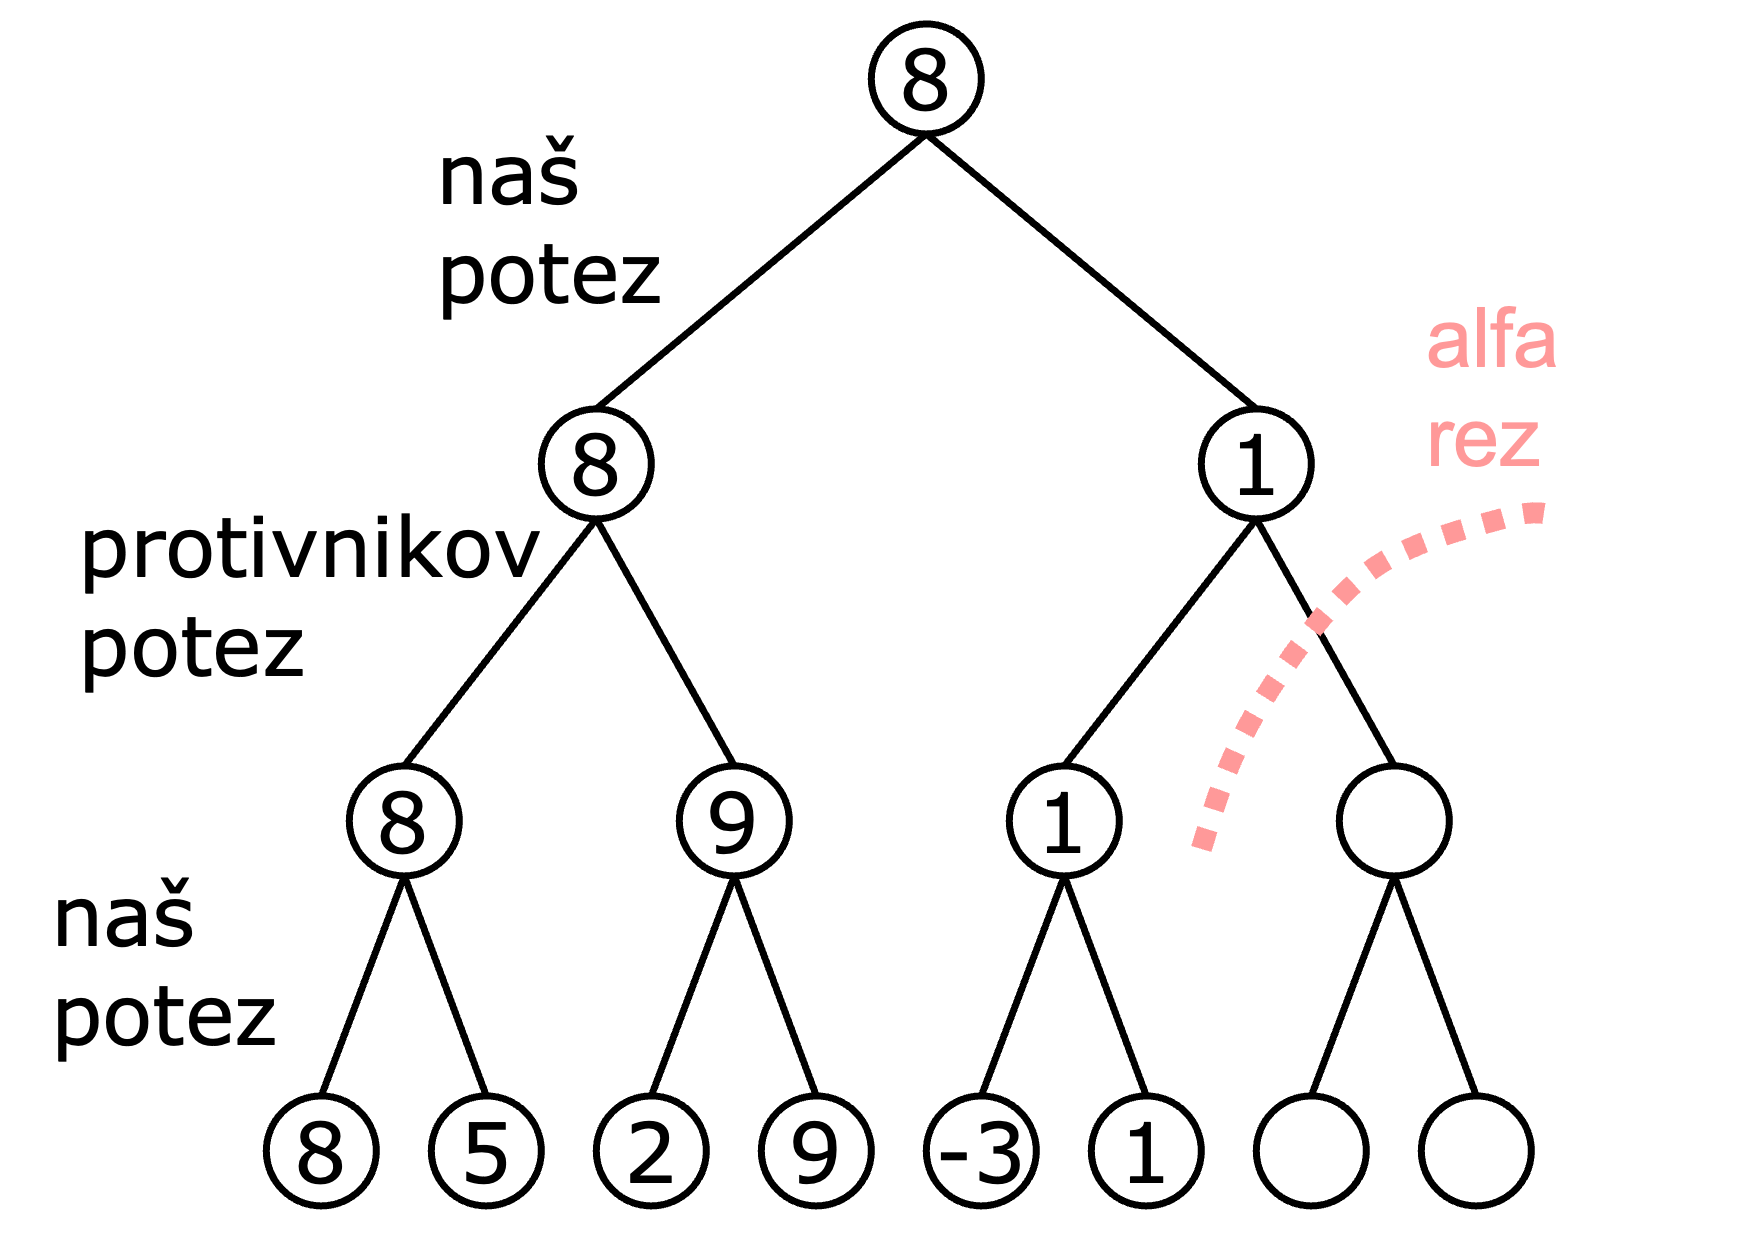
\includegraphics[width=7cm]{prj-01-pic11.png}
    \end{center}
  \end{columns}
\end{frame}

\begin{frame}[fragile]
  \frametitle{Radimo alfa rez kada:}
  \begin{columns}
    \column{8cm}
    \begin{itemize}
      \item posmatramo čvor posle koga igra protivnik i
      \item roditelj ima vrednost i
      \item vrednost u čvoru je manja od roditelja i
      \item čvor ima decu koju možemo rezati
    \end{itemize}
    \column{8cm}
    \begin{center}
      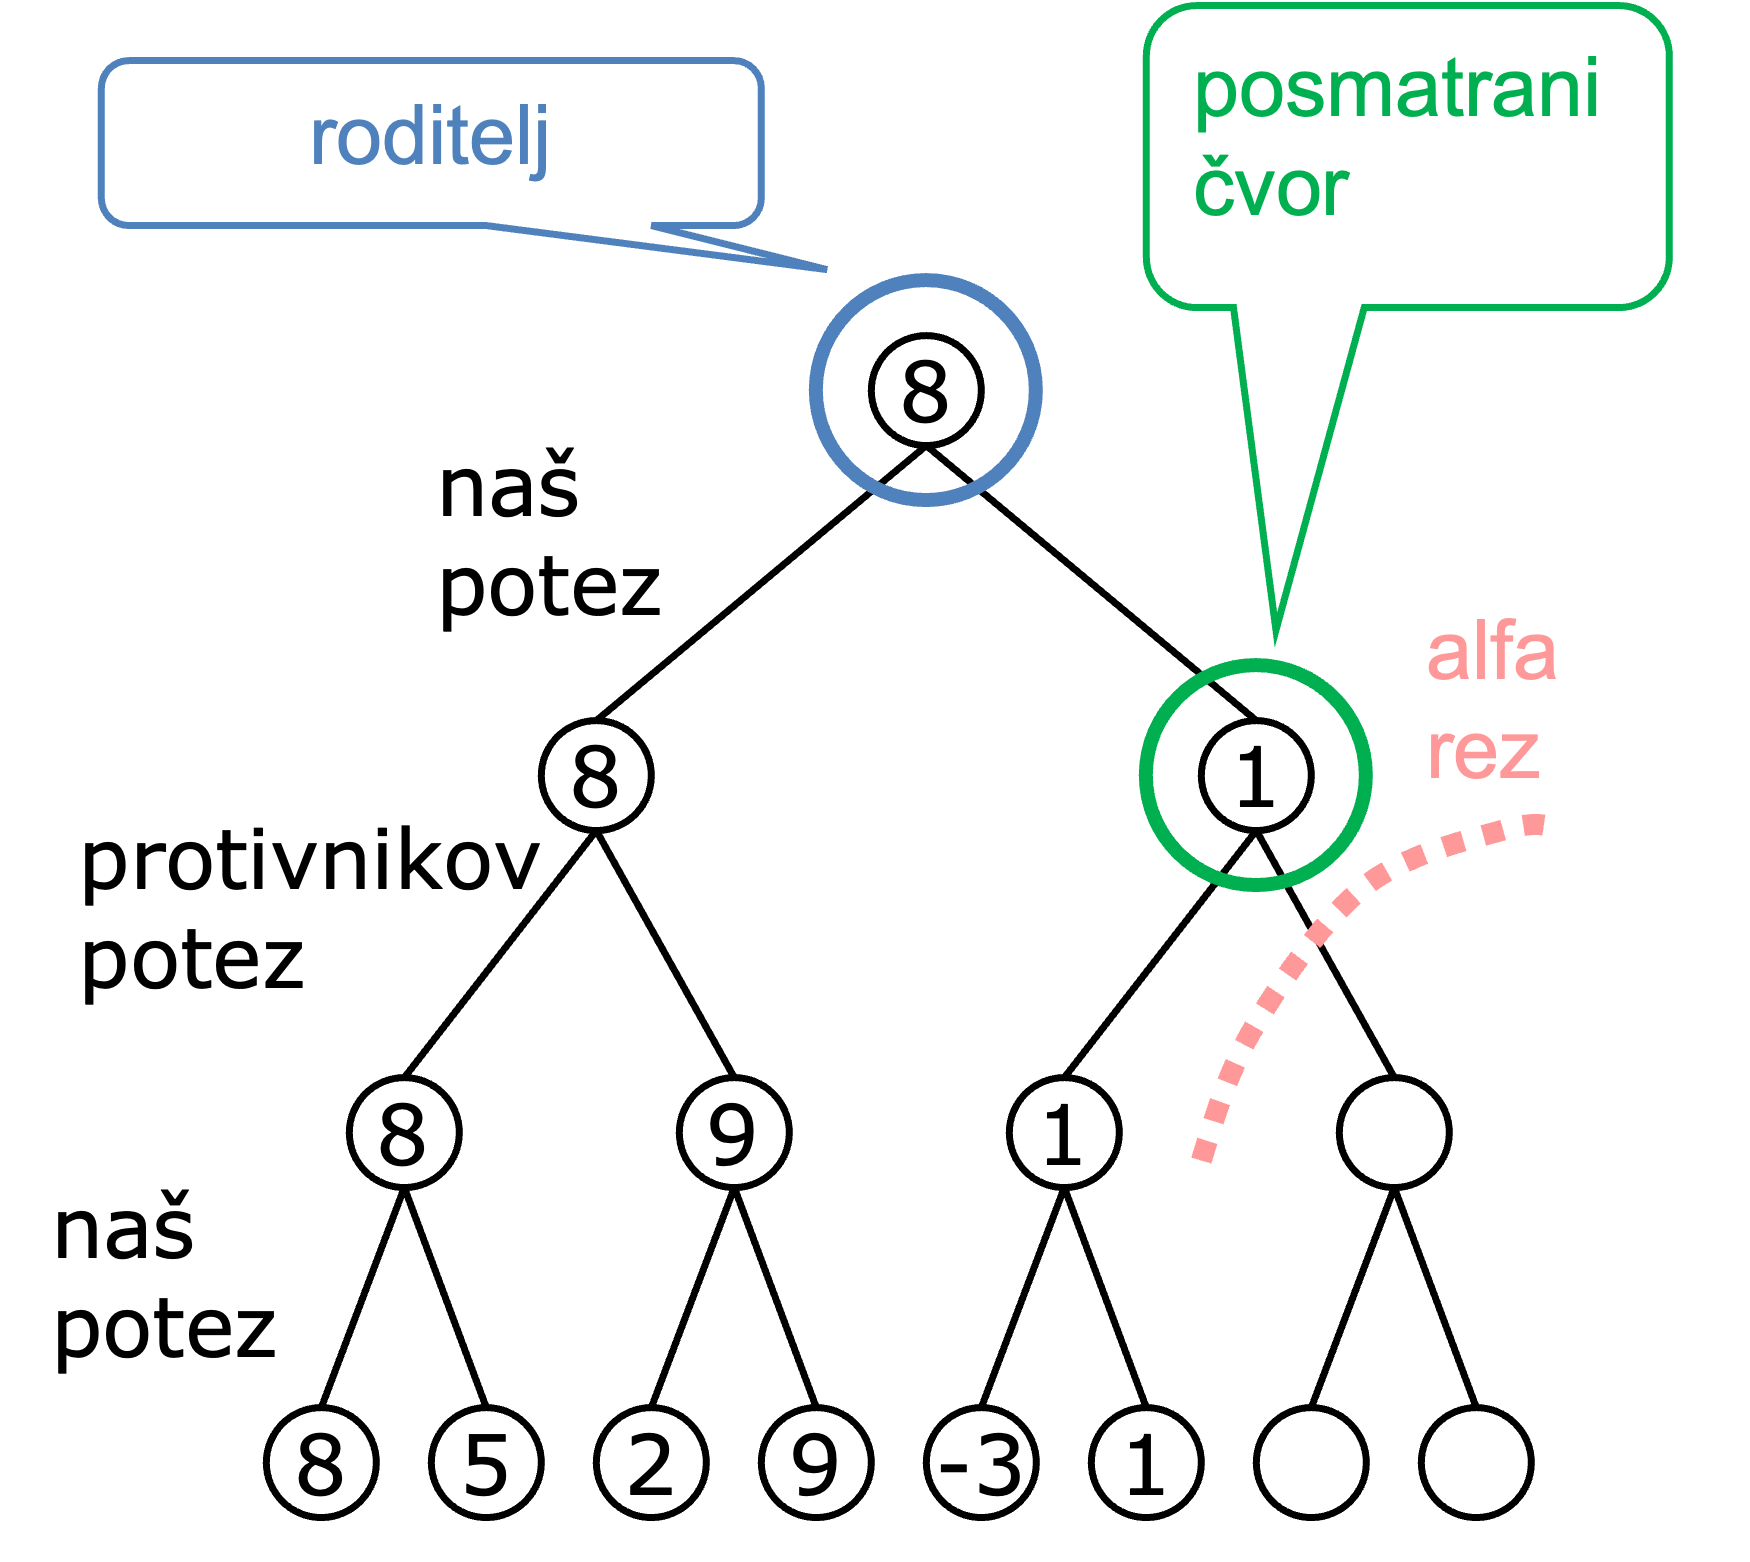
\includegraphics[width=7cm]{prj-01-pic12.png}
    \end{center}
  \end{columns}
\end{frame}

\begin{frame}[fragile]
  \frametitle{Beta rez}
  \begin{itemize}
    \item \textbf{\myred{alfa rez}} radimo kada
    \begin{itemize}
      \item protivnik je na potezu
      \item imamo vrednost za roditelja
      \item roditelj ima \textbf{veću} vrednost nego posmatrani čvor
      \item posmatrani čvor ima decu koju nismo prošli
    \end{itemize}
    \item \textbf{\myred{beta rez}} radimo kada
    \begin{itemize}
      \item mi smo na potezu
      \item imamo vrednost za roditelja
      \item roditelj ima \textbf{manju} vrednost nego posmatrani čvor
      \item posmatrani čvor ima decu koju nismo prošli
    \end{itemize}
  \end{itemize}
\end{frame}

\begin{frame}[fragile]
  \frametitle{Beta rez}
  \begin{itemize}
    \item protivnikov alfa rez je za nas beta rez
    \begin{itemize}
      \item gledamo iz perspektive protivnika
    \end{itemize}
    \item pretpostavljamo da je protivnik racionalan i koristi istu ili sličnu heuristiku
    \item čak i da je različita, to je najbolje što možemo
  \end{itemize}
\end{frame}

\begin{frame}[fragile]
  \frametitle{Značaj rezanja}
  \begin{itemize}
    \item ako možemo obići celo stablo znamo tačno kako treba da igramo
    \item što dublje istražimo to bolje
    \item ako odrežemo delove stabla možemo ići dublje na drugoj strani
    \item što je rez bliži korenu tim bolje
    \item ako broj čvorova u nivoima raste eksponencijalno, dobitak je veliki
  \end{itemize}
\end{frame}

\begin{frame}[fragile]
  \frametitle{Rezanje i heuristika}
  \begin{itemize}
    \item primeni heuristiku na svaki čvor
    \begin{itemize}
      \item ne samo na čvorove najnižeg nivoa
    \end{itemize}
    \item idi prvo niz \textbf{najbolje} čvorove
    \begin{itemize}
      \item ,,najbolji`` zavisi od igrača koji je na potezu -- najbolji za njega
    \end{itemize}
  \end{itemize}
\end{frame}

\begin{frame}[fragile]
  \frametitle{Balans performansi}
  \begin{itemize}
    \item dublji obilazak stabla traje duže
    \item preciznija heuristika se izračunava duže
    \item treba naći balans između kvaliteta heuristike i dubine obilaska stabla
  \end{itemize}
\end{frame}

\begin{frame}[fragile]
  \frametitle{Mice / Nine men's morris}
  \begin{center}
    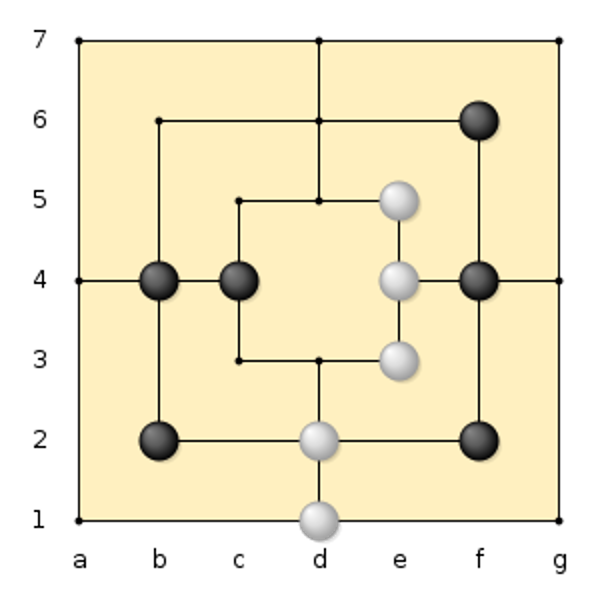
\includegraphics[width=7cm]{prj-01-pic13.png}
  \end{center}
\end{frame}

\begin{frame}[fragile]
  \frametitle{Mice}
  \begin{itemize}
    \item 2 igrača (beli, crni) po 9 figura
    \item položaj figura u čvorovima mreže
    \item kretanje figura duž linija (po 1 korak)
    \item igru gubi onaj koji ostane sa 2 figure ili ne može više da se kreće
  \end{itemize}
\end{frame}

\begin{frame}[fragile]
  \frametitle{Mice}
  \begin{itemize}
    \item kada igrač postavi 3 figure u nizu ima pravo da ukloni jednu protivničku figuru
    \item može da bira koju će ukloniti
    \item ne sme ukloniti one koje su u nizu od 3
    \begin{itemize}
      \item osim ako su sve protivničke figure u nizu od 3
    \end{itemize}
  \end{itemize}
\end{frame}

\begin{frame}[fragile]
  \frametitle{Faza 1: postavljanje figura}
  \begin{itemize}
    \item igra počinje sa praznom tablom
    \item igrači naizmenično postavljaju svojih 9 figura na slobodna polja na tabli
    \item ukoliko igrač formira niz od 3 figure, ima pravo da ukloni jednu protivničku figuru
    \begin{itemize}
      \item protivnička figura koja se uklanja ne sme biti deo protivničkog niza od 3 figure
      \begin{itemize}
        \item osim u slučaju da su sve protivničke figure u nizu od 3
      \end{itemize}
    \end{itemize}
  \end{itemize}
\end{frame}

\begin{frame}[fragile]
  \frametitle{Faza 2: kretanje}
  \begin{itemize}
    \item igrači naizmenično igraju po jedan potez
    \item potez predstavlja pomeranje svoje figure na susedno slobodno mesto
    \item cilj kretanja je da se formira niz od 3 svoje figure kada je moguće ukloniti jednu protivničku figuru
    \item kada jedan od igrača ostane sa 3 figure na tabli, prelazi se na fazu 3
  \end{itemize}
\end{frame}

\begin{frame}[fragile]
  \frametitle{Faza 3: preskakanje}
  \begin{itemize}
    \item figure se mogu pomeriti na bilo koju slobodnu poziciju na tabli, uključujući i preskakanje \\ \ \\ \ \\
    \item \textit{napomena}: za ovu igru su kroz istoriju formirana različita pravila, pri čemu često faza 3 u igri ne postoji
  \end{itemize}
\end{frame}

\begin{frame}[fragile]
  \frametitle{Heuristika za mice $_1$}
  \begin{columns}
    \column{8cm}
    \begin{itemize}
      \item \#1 vezane 3 figure
      \begin{itemize}
        \item +1 ako smo vezali 3 figure u prethodnom potezu
        \item -1 ako je protivnik to uradio
        \item 0 inače
      \end{itemize}
    \end{itemize}
    \column{8cm}
    \begin{center}
      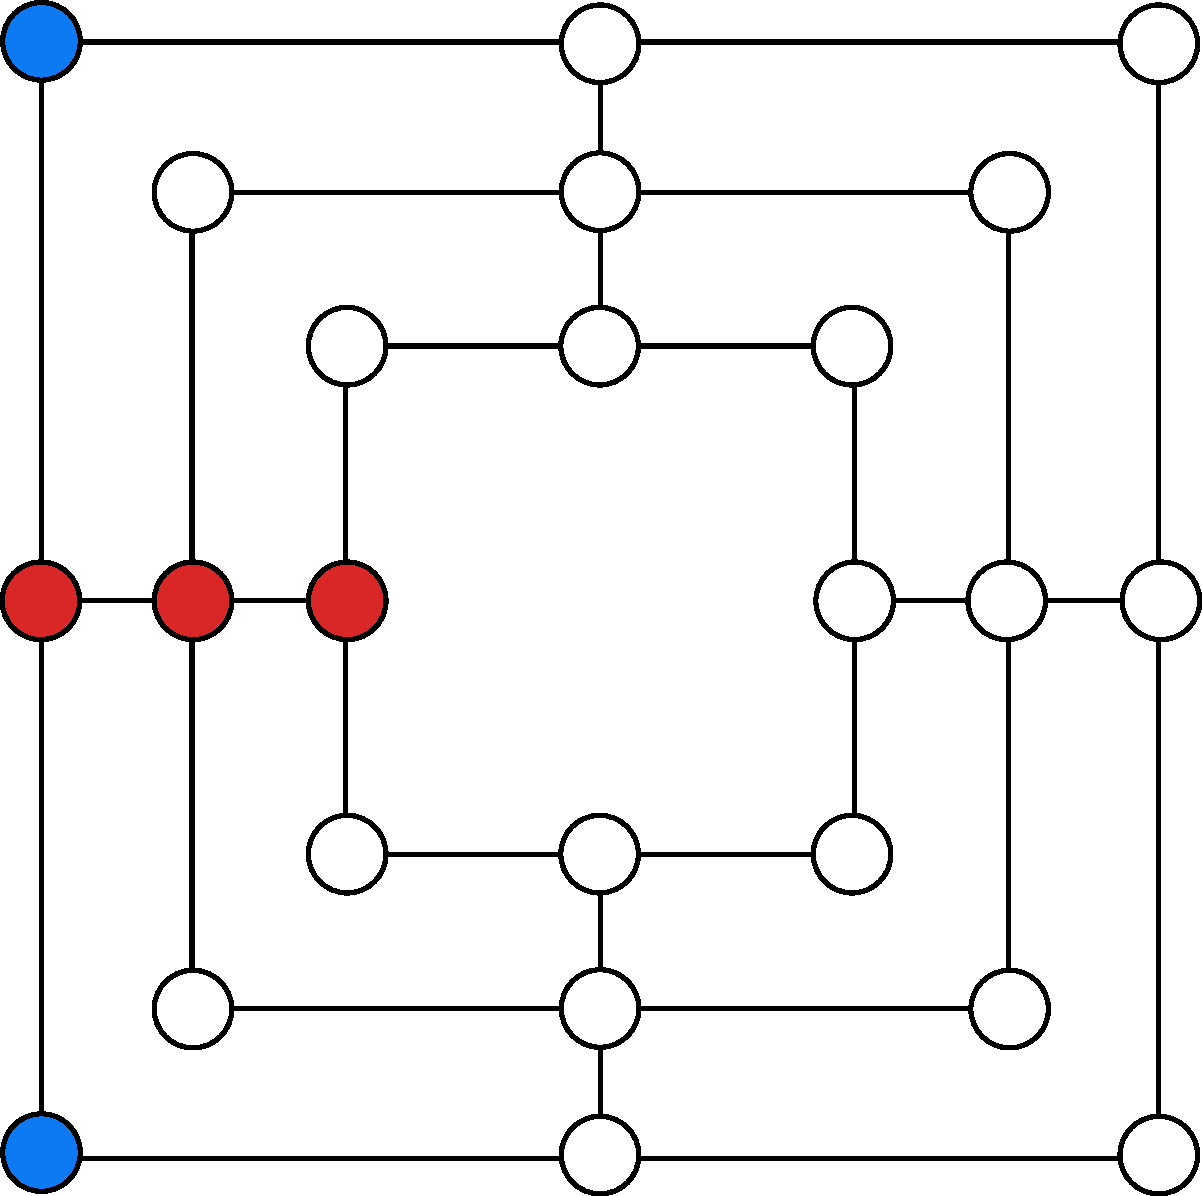
\includegraphics[width=5cm]{prj-01-pic14.pdf}
    \end{center}
  \end{columns}
\end{frame}

\begin{frame}[fragile]
  \frametitle{Heuristika za mice $_2$}
  \begin{itemize}
    \item \#2 razlika broja vezanih trojki koju imamo mi i protivnik
  \end{itemize}
\end{frame}

\begin{frame}[fragile]
  \frametitle{Heuristika za mice $_3$}
  \begin{itemize}
    \item \#3 razlika broja blokiranih protivničkih figura
  \end{itemize}
  \begin{center}
    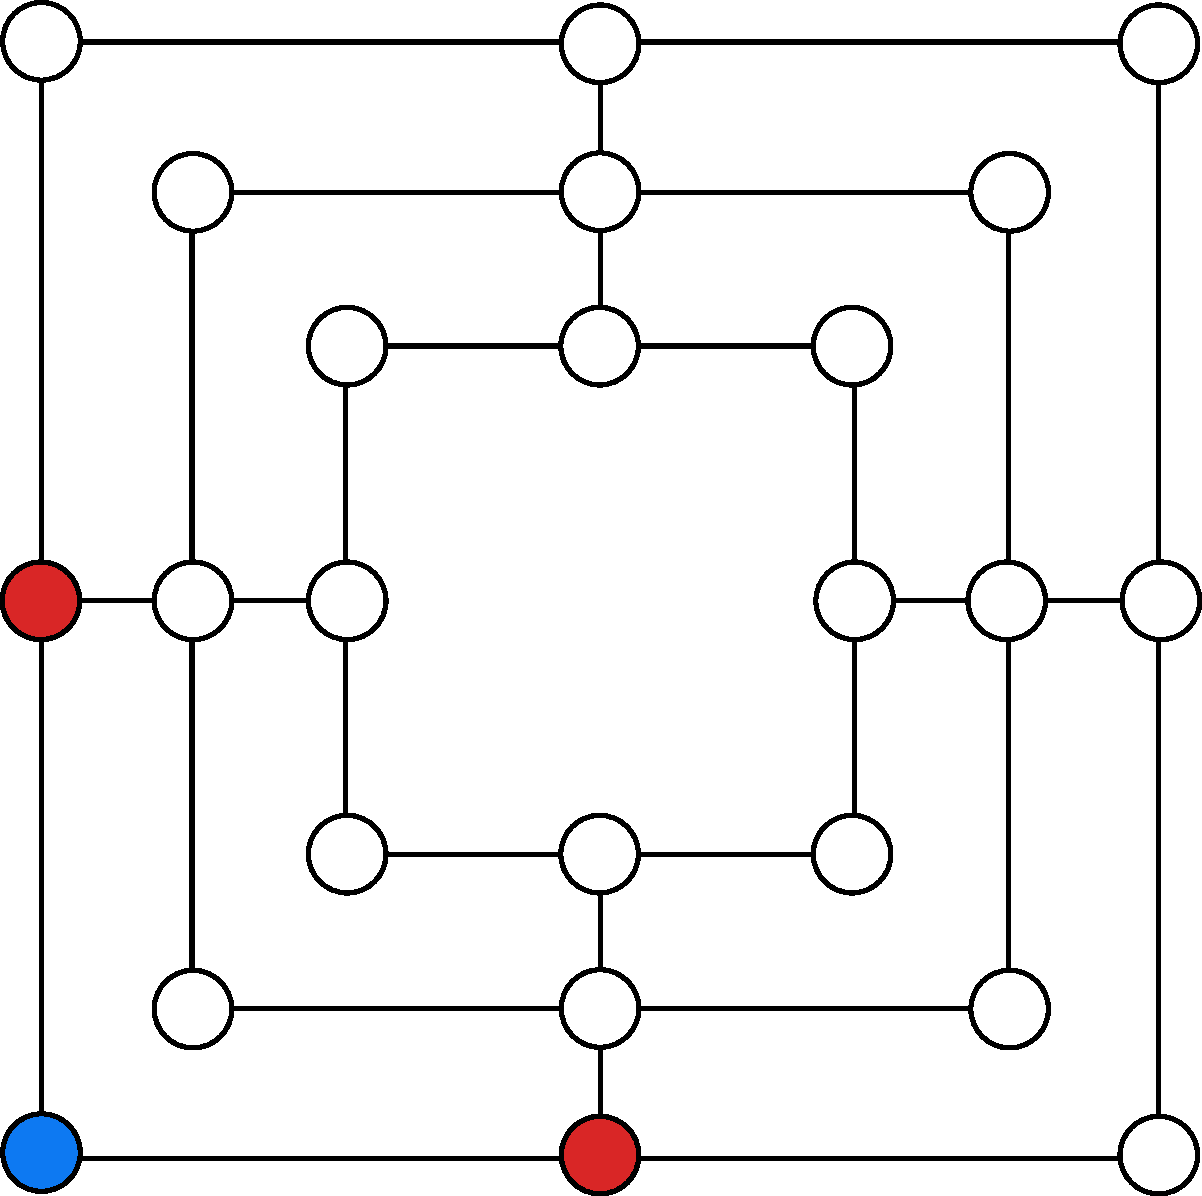
\includegraphics[width=5cm]{prj-01-pic15.pdf}
  \end{center}
\end{frame}

\begin{frame}[fragile]
  \frametitle{Heuristika za mice $_4$}
  \begin{itemize}
    \item \#4 razlika broja naših i protivničkih figura
  \end{itemize}
\end{frame}

\begin{frame}[fragile]
  \frametitle{Heuristika za mice $_5$}
  \begin{itemize}
    \item \#5 razlika broja vezanih dvojki
    \begin{itemize}
      \item dvojka: položaj u kome nam nedostaje jedna figura za trojku
    \end{itemize}
  \end{itemize}
  \begin{center}
    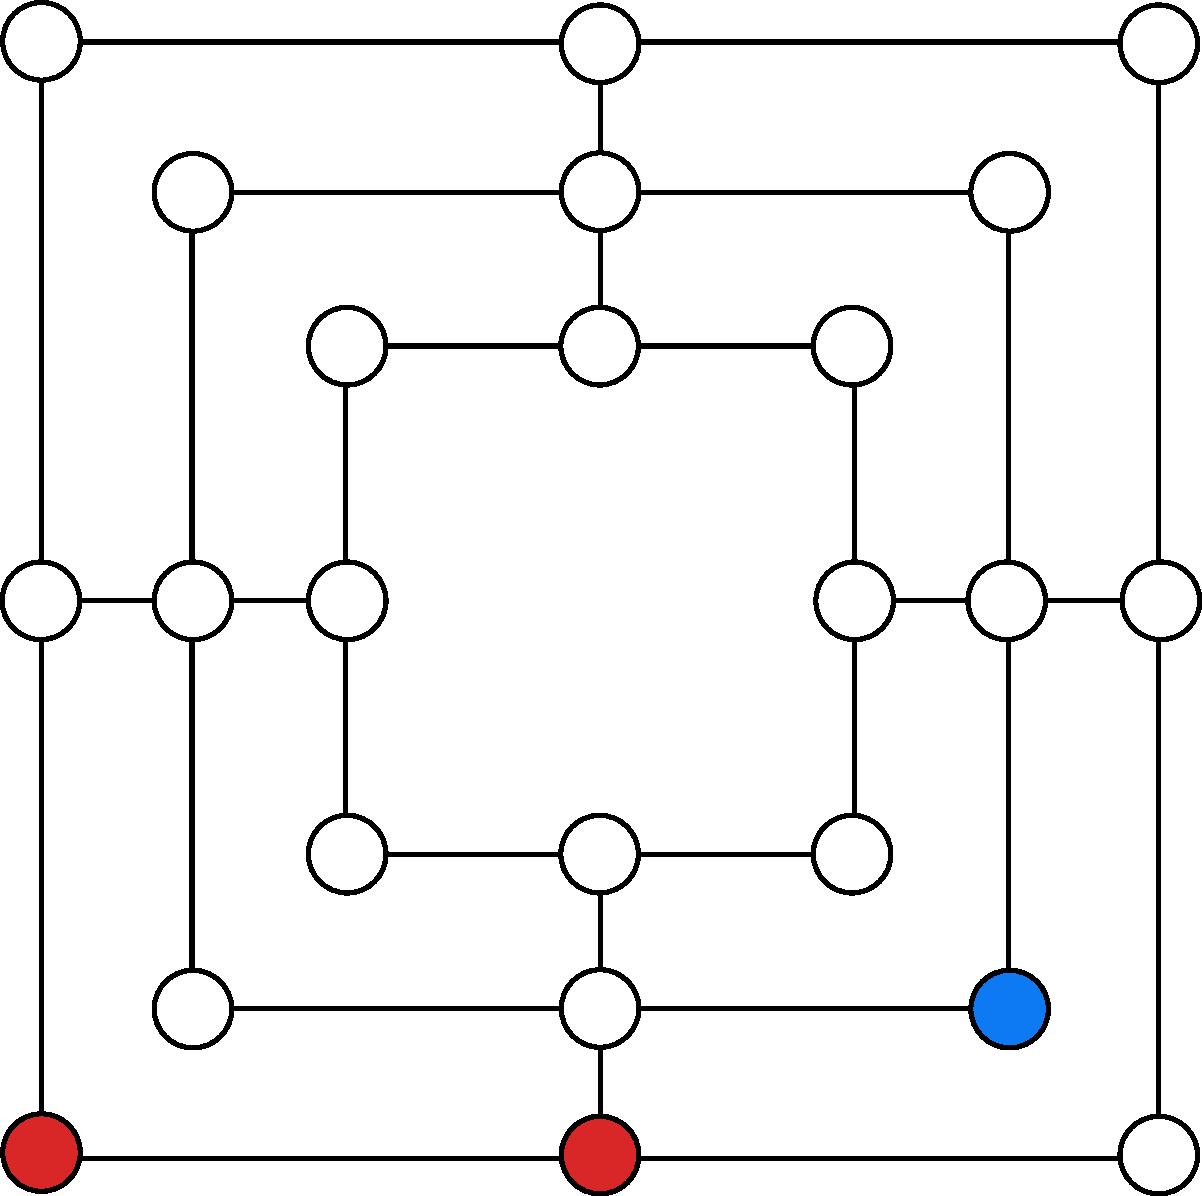
\includegraphics[width=5cm]{prj-01-pic16.pdf}
  \end{center}
\end{frame}

\begin{frame}[fragile]
  \frametitle{Heuristika za mice $_6$}
  \begin{itemize}
    \item \#6 razlika broja trojki
    \begin{itemize}
      \item trojka: postoji 2 načina za pravljenje vezane trojke
    \end{itemize}
  \end{itemize}
  \begin{center}
    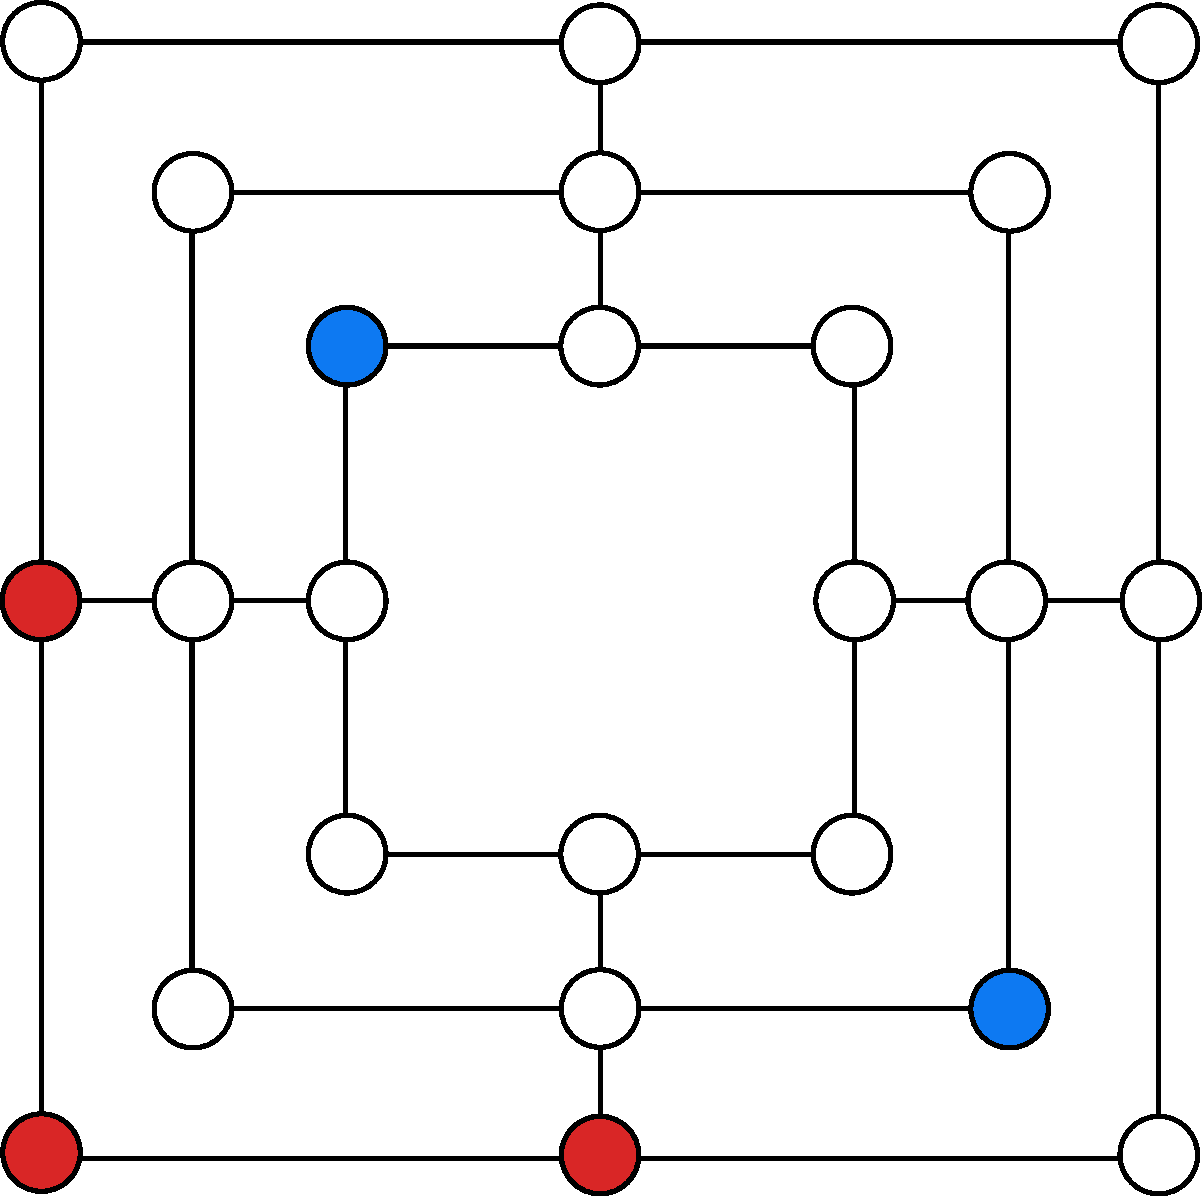
\includegraphics[width=5cm]{prj-01-pic17.pdf}
  \end{center}
\end{frame}

\begin{frame}[fragile]
  \frametitle{Heuristika za mice $_7$}
  \begin{itemize}
    \item \#7 razlika broja duplih vezanih trojki
    \begin{itemize}
      \item dupla vezana trojka: dve vezane trojke koje imaju zajedničku figuru
    \end{itemize}
  \end{itemize}
  \begin{center}
    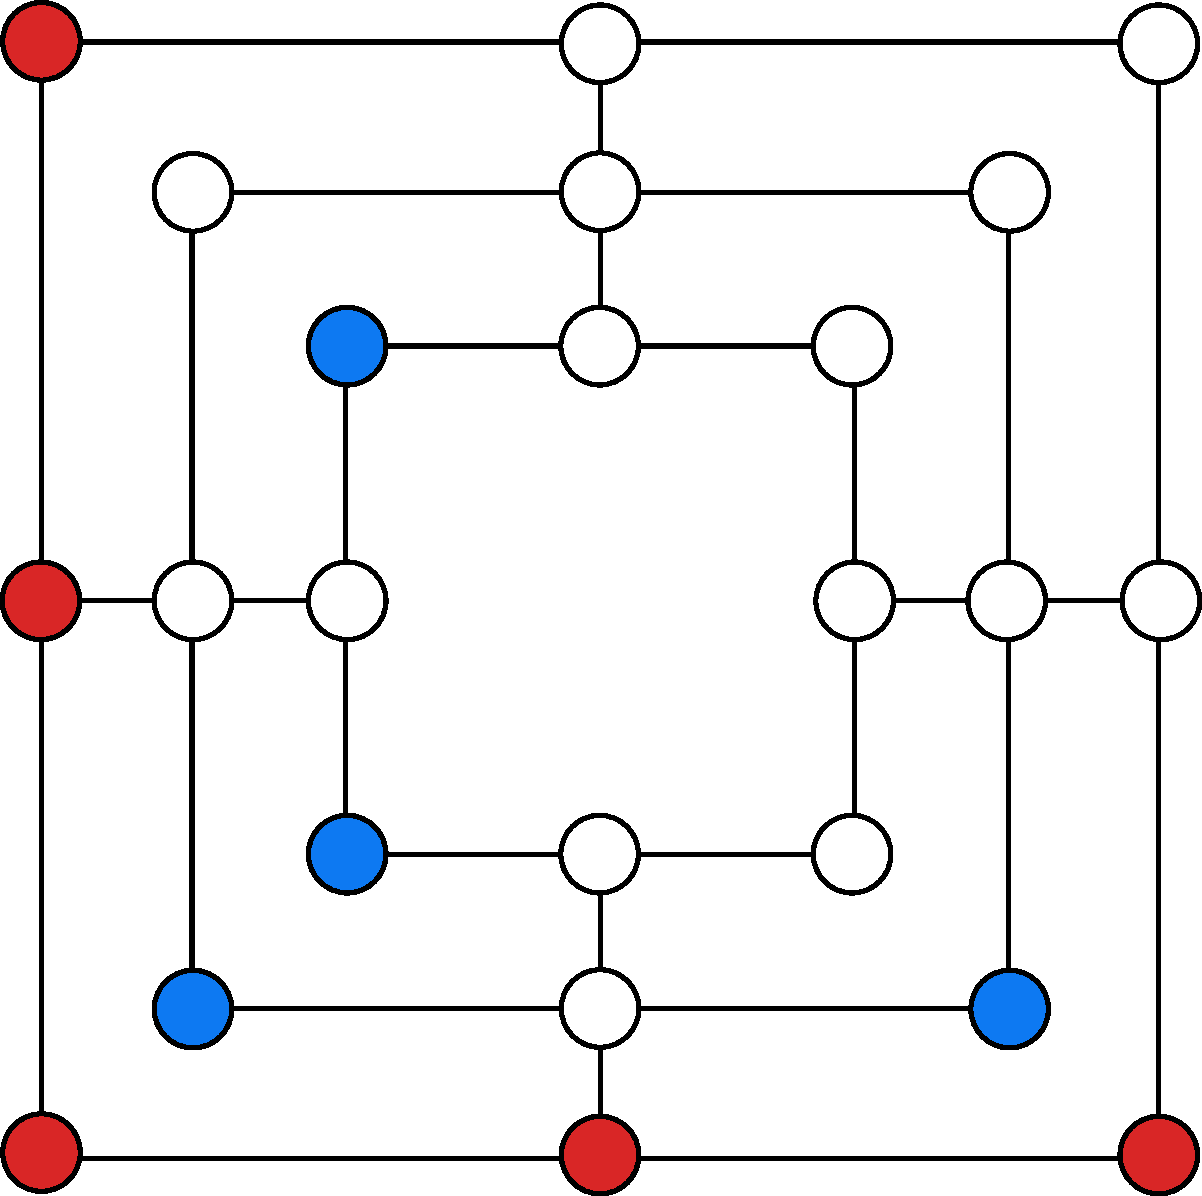
\includegraphics[width=5cm]{prj-01-pic18.pdf}
  \end{center}
\end{frame}

\begin{frame}[fragile]
  \frametitle{Heuristika za mice $_8$}
  \begin{itemize}
    \item \#8 pobednički raspored
    \begin{itemize}
      \item +1 ako je pobeda naša
      \item -1 ako je pobeda protivnikova
      \item 0 inače
    \end{itemize}
  \end{itemize}
\end{frame}

\begin{frame}[fragile]
  \frametitle{Heuristika za mice}
  \begin{itemize}
    \item kako povezati ove kriterijume?
    \begin{itemize}
      \item \url{http://www.dasconference.ro/papers/2008/B7.pdf} \\ \ \\
    \end{itemize}
    \item obilazak stabla
    \begin{itemize}
      \item max dubina?
      \item niz koliko dece?
    \end{itemize}
  \end{itemize}
\end{frame}

\end{document}
